
\documentclass[letterpaper,hide notes,xcolor={table,svgnames},pdftex,10pt]{beamer}
\def\showexamples{t}

\usecolortheme{crane}
\setbeamertemplate{navigation symbols}{}

\usetheme{MyPittsburgh}
\usepackage{hyperref}
\usepackage{graphicx,xspace}
\usepackage[normalem]{ulem}
\usepackage{multicol}
\usepackage{amsmath,amssymb,amsthm,graphicx,xspace}
\newcommand\SF[1]{$\bigstar$\footnote{SF: #1}}

\usepackage[sfdefault,lf]{carlito}
\usepackage[T1]{fontenc}
\usepackage[scaled]{beramono}
\usepackage{tikzpagenodes}
\newcommand{\Rplus}{\protect\hspace{-.1em}\protect\raisebox{.35ex}{\small{\small\textbf{+}}}}
\newcommand{\Cpp}{\mbox{C\Rplus\Rplus}\xspace}

\newcounter{tmpnumSlide}
\newcounter{tmpnumNote}

\newcommand\mnote[1]{%
	\addtocounter{tmpnumSlide}{1}
	\ifdefined\showcues {~\tiny\fbox{\arabic{tmpnumSlide}}}\fi
	\note{\setlength{\parskip}{1ex}\addtocounter{tmpnumNote}{1}\textbf{\Large \arabic{tmpnumNote}:} {#1\par}}}

\newcommand\mmnote[1]{\note{\setlength{\parskip}{1ex}#1\par}}


\newcommand\mquestion[2]{{~\color{red}\fbox{?}}\note{\setlength{\parskip}{1ex}\par{\Large \textbf{?}} #1} \note{\setlength{\parskip}{1ex}\par{\Large \textbf{A}} #2\par}\ifdefined \presentationonly \pause \fi}

\newcommand\blackboard[1]{%
	\ifdefined   \showblackboard
		{#1}
	\else {\begin{center} \fbox{\colorbox{blue!30}{%
						\begin{minipage}{.95\linewidth}%
							\hspace{\stretch{1}} Some space intentionally left blank; done at the blackboard.%
						\end{minipage}}}\end{center}}%
	\fi%
}

\usepackage{listings}
\lstset{%
	keywordstyle=\bfseries,
	aboveskip=15pt,
	belowskip=15pt,
	captionpos=b,
	identifierstyle=\ttfamily,
	frame=lines,
	numbers=left, basicstyle=\scriptsize, numberstyle=\tiny, stepnumber=0, numbersep=2pt}

\usepackage{siunitx}
\newcommand\sius[1]{\num[group-separator = {,}]{#1}\si{\micro\second}}
\newcommand\sims[1]{\num[group-separator = {,}]{#1}\si{\milli\second}}
\newcommand\sins[1]{\num[group-separator = {,}]{#1}\si{\nano\second}}
\sisetup{group-separator = {,}, group-digits = true}

%% -------------------- tikz --------------------
\usepackage{tikz}
\usetikzlibrary{positioning}
\usetikzlibrary{arrows,backgrounds,automata,decorations.shapes,decorations.pathmorphing,decorations.markings,decorations.text}

\tikzstyle{place}=[circle,draw=blue!50,fill=blue!20,thick, inner sep=0pt,minimum size=6mm]
\tikzstyle{transition}=[rectangle,draw=black!50,fill=black!20,thick, inner sep=0pt,minimum size=4mm]

\tikzstyle{block}=[rectangle,draw=black, thick, inner sep=5pt]
\tikzstyle{bullet}=[circle,draw=black, fill=black, thin, inner sep=2pt]

\tikzstyle{pre}=[<-,shorten <=1pt,>=stealth',semithick]
\tikzstyle{post}=[->,shorten >=1pt,>=stealth',semithick]
\tikzstyle{bi}=[<->,shorten >=1pt,shorten <=1pt, >=stealth',semithick]

\tikzstyle{mut}=[-,>=stealth',semithick]

\tikzstyle{treereset}=[dashed,->, shorten >=1pt,>=stealth',thin]

\usepackage{ifmtarg}
\usepackage{xifthen}
\makeatletter
% new counter to now which frame it is within the sequence
\newcounter{multiframecounter}
% initialize buffer for previously used frame title
\gdef\lastframetitle{\textit{undefined}}
% new environment for a multi-frame
\newenvironment{multiframe}[1][]{%
	\ifthenelse{\isempty{#1}}{%
		% if no frame title was set via optional parameter,
		% only increase sequence counter by 1
		\addtocounter{multiframecounter}{1}%
	}{%
		% new frame title has been provided, thus
		% reset sequence counter to 1 and buffer frame title for later use
		\setcounter{multiframecounter}{1}%
		\gdef\lastframetitle{#1}%
	}%
	% start conventional frame environment and
	% automatically set frame title followed by sequence counter
	\begin{frame}%
		\frametitle{\lastframetitle~{\normalfont(\arabic{multiframecounter})}}%
		}{%
	\end{frame}%
}
\makeatother

\makeatletter
\newdimen\tu@tmpa%
\newdimen\ydiffl%
\newdimen\xdiffl%
\newcommand\ydiff[2]{%
	\coordinate (tmpnamea) at (#1);%
	\coordinate (tmpnameb) at (#2);%
	\pgfextracty{\tu@tmpa}{\pgfpointanchor{tmpnamea}{center}}%
	\pgfextracty{\ydiffl}{\pgfpointanchor{tmpnameb}{center}}%
	\advance\ydiffl by -\tu@tmpa%
}
\newcommand\xdiff[2]{%
	\coordinate (tmpnamea) at (#1);%
	\coordinate (tmpnameb) at (#2);%
	\pgfextractx{\tu@tmpa}{\pgfpointanchor{tmpnamea}{center}}%
	\pgfextractx{\xdiffl}{\pgfpointanchor{tmpnameb}{center}}%
	\advance\xdiffl by -\tu@tmpa%
}
\makeatother
\newcommand{\copyrightbox}[3][r]{%
	\begin{tikzpicture}%
		\node[inner sep=0pt,minimum size=2em](ciimage){#2};
		\usefont{OT1}{phv}{n}{n}\fontsize{4}{4}\selectfont
		\ydiff{ciimage.south}{ciimage.north}
		\xdiff{ciimage.west}{ciimage.east}
		\ifthenelse{\equal{#1}{r}}{%
			\node[inner sep=0pt,right=1ex of ciimage.south east,anchor=north west,rotate=90]%
			{\raggedleft\color{black!50}\parbox{\the\ydiffl}{\raggedright{}#3}};%
		}{%
			\ifthenelse{\equal{#1}{l}}{%
				\node[inner sep=0pt,right=1ex of ciimage.south west,anchor=south west,rotate=90]%
				{\raggedleft\color{black!50}\parbox{\the\ydiffl}{\raggedright{}#3}};%
			}{%
				\node[inner sep=0pt,below=1ex of ciimage.south west,anchor=north west]%
				{\raggedleft\color{black!50}\parbox{\the\xdiffl}{\raggedright{}#3}};%
			}
		}
	\end{tikzpicture}
}


%% --------------------

%\usepackage[excludeor]{everyhook}
%\PushPreHook{par}{\setbox0=\lastbox\llap{MUH}}\box0}

%\vspace*{\stretch{1}

%\setbox0=\lastbox \llap{\textbullet\enskip}\box0}

\setlength{\parskip}{\fill}

\newcommand\noskips{\setlength{\parskip}{1ex}}
\newcommand\doskips{\setlength{\parskip}{\fill}}

\newcommand\xx{\par\vspace*{\stretch{1}}\par}
\newcommand\xxs{\par\vspace*{2ex}\par}
\newcommand\tuple[1]{\langle #1 \rangle}
\newcommand\code[1]{{\sf \footnotesize #1}}
\newcommand\ex[1]{\uline{Example:} \ifdefined \presentationonly \pause \fi
	\ifdefined\showexamples#1\xspace\else{\uline{\hspace*{2cm}}}\fi}

\newcommand\ceil[1]{\lceil #1 \rceil}


\AtBeginSection[]
{
	\begin{frame}
		\frametitle{Outline}
		\tableofcontents[currentsection]
	\end{frame}
}



\pgfdeclarelayer{edgelayer}
\pgfdeclarelayer{nodelayer}
\pgfsetlayers{edgelayer,nodelayer,main}

\tikzstyle{none}=[inner sep=0pt]
\tikzstyle{rn}=[circle,fill=Red,draw=Black,line width=0.8 pt]
\tikzstyle{gn}=[circle,fill=Lime,draw=Black,line width=0.8 pt]
\tikzstyle{yn}=[circle,fill=Yellow,draw=Black,line width=0.8 pt]
\tikzstyle{empty}=[circle,fill=White,draw=Black]
\tikzstyle{bw} = [rectangle, draw, fill=blue!20,
text width=4em, text centered, rounded corners, minimum height=2em]

\newcommand{\CcNote}[1]{% longname
	This work is licensed under the \textit{Creative Commons #1 3.0 License}.%
}
\newcommand{\CcImageBy}[1]{%
	\includegraphics[scale=#1]{creative_commons/cc_by_30.pdf}%
}
\newcommand{\CcImageSa}[1]{%
	\includegraphics[scale=#1]{creative_commons/cc_sa_30.pdf}%
}
\newcommand{\CcImageNc}[1]{%
	\includegraphics[scale=#1]{creative_commons/cc_nc_30.pdf}%
}
\newcommand{\CcGroupBySa}[2]{% zoom, gap
	\CcImageBy{#1}\hspace*{#2}\CcImageNc{#1}\hspace*{#2}\CcImageSa{#1}%
}
\newcommand{\CcLongnameByNcSa}{Attribution-NonCommercial-ShareAlike}

\newenvironment{changemargin}[1]{% 
	\begin{list}{}{% 
		\setlength{\topsep}{0pt}% 
		\setlength{\leftmargin}{#1}% 
		\setlength{\rightmargin}{1em}
		\setlength{\listparindent}{\parindent}% 
		\setlength{\itemindent}{\parindent}% 
		      \setlength{\parsep}{\parskip}% 
		      }% 
		\item[]}{\end{list}}




\title{Lecture 9 --- Memory: Segmentation \& Paging }

\author{Jeff Zarnett \\ \small \texttt{jzarnett@uwaterloo.ca}}
\institute{Department of Electrical and Computer Engineering \\
  University of Waterloo}
\date{\today}


\begin{document}

\begin{frame}
  \titlepage

 \end{frame}

\begin{frame}
\frametitle{Big Memory for Big Computer}

Let's think about memory management in a larger (desktop/laptop) system.


\end{frame}


\begin{frame}
\frametitle{Memory Segmentation}

You've been repeatedly told that memory is a linear array of bytes. 

You have also been told that there's the stack and the heap, libraries and instructions.

\begin{center}
	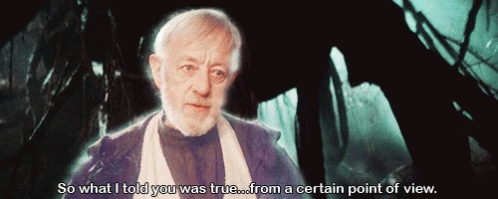
\includegraphics[width=\textwidth]{images/pov.jpg}
\end{center}

 \end{frame}



\begin{frame}
\frametitle{Memory Segmentation}

Both are true; they are views of memory at different levels of abstraction. 

Each of the elements such as the stack, the heap, the standard C library, et cetera, are known as \alert{segments}.

\begin{center}
	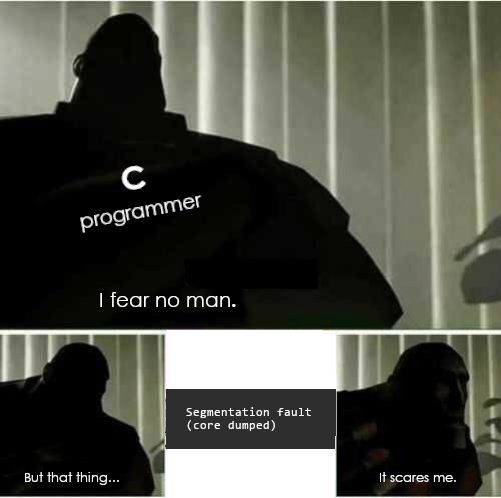
\includegraphics[width=0.4\textwidth]{images/segfault.png}
\end{center}


\end{frame}

\begin{frame}
\frametitle{Memory Segmentation}

Programmers do not necessarily give much thought to whether variables are allocated on the stack or the heap.

Or where program instructions appear in memory. 

In many cases it does not matter, though C programmers are well advised to know the difference.


\end{frame}

\begin{frame}
\frametitle{Memory Segments}

A full program has a collection of different-sized segments, made by the compiler.

\begin{enumerate}
	\item The code (instructions).
	\item Global variables.
	\item The heap.
	\item The stack (one per thread).
	\item The standard C library.
\end{enumerate}

\end{frame}

\begin{frame}
\frametitle{Segments from the Programmer's Perspective}

\begin{center}
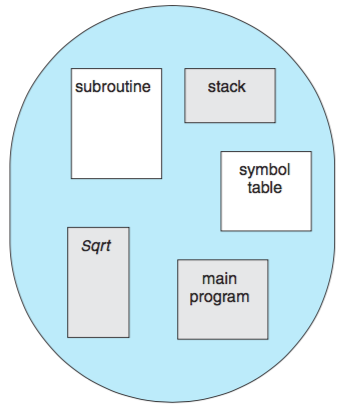
\includegraphics[width=0.55\textwidth]{images/segments.png}
\end{center}


\end{frame}

\begin{frame}
\frametitle{Thinking about Segments}

Rather than thinking about memory as just a pure address, we can think of it as a tuple: \textit{$<$segment, offset$>$}. 

Given that, we need an implementation to map these tuples into memory addresses. 

The mapping has a segment table.

\end{frame}

\begin{frame}
\frametitle{Thinking about Segments}

Each entry in the table contains two values: the base and the limit.

So there will be some addition involved as well as a comparison to see if the address lies within that range.

\end{frame}

\begin{frame}
\frametitle{Segment Table: Hardware}

Memory accesses are such a common operation that we will need another rescue from the hardware folks to make this not painfully slow.

\begin{center}
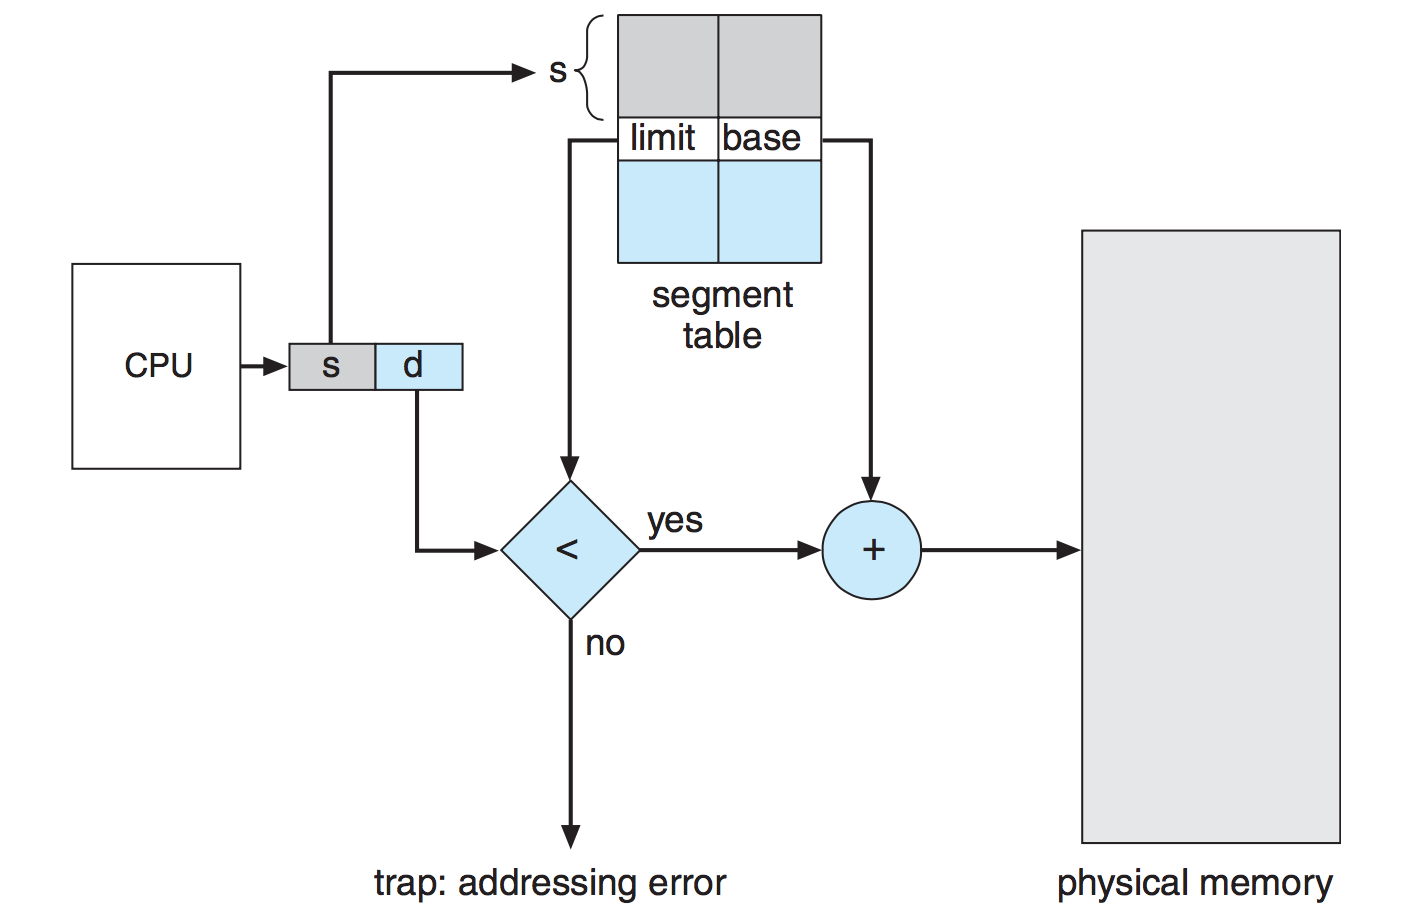
\includegraphics[width=0.75\textwidth]{images/segmentation-hardware.png}
\end{center}

\end{frame}

\begin{frame}
\frametitle{Segmentation: Contiguous}

With segmentation, memory need no longer be contiguous. 

We can allocate different parts of the program in different segments. 

Different segments can be located in different areas of memory.

(Want to find out where something is? Use the \texttt{\&} [address-of] operator...)


\end{frame}

\begin{frame}
\frametitle{Paging}

Fixed \& variable sized partitions suffer from fragmentation, external or internal. 

Divide memory up into small, fixed-size chunks of equal size, called \alert{frames}. 

Divide each process's memory into chunks the same size as a frame: \alert{pages}. 

Then a page can be assigned to a frame. 

A frame may be empty or may have exactly one page in it. 


\end{frame}

\begin{frame}
\frametitle{Paging: Picture Frame}

Imagine, as an analogy, a simple picture frame. 

\begin{center}
	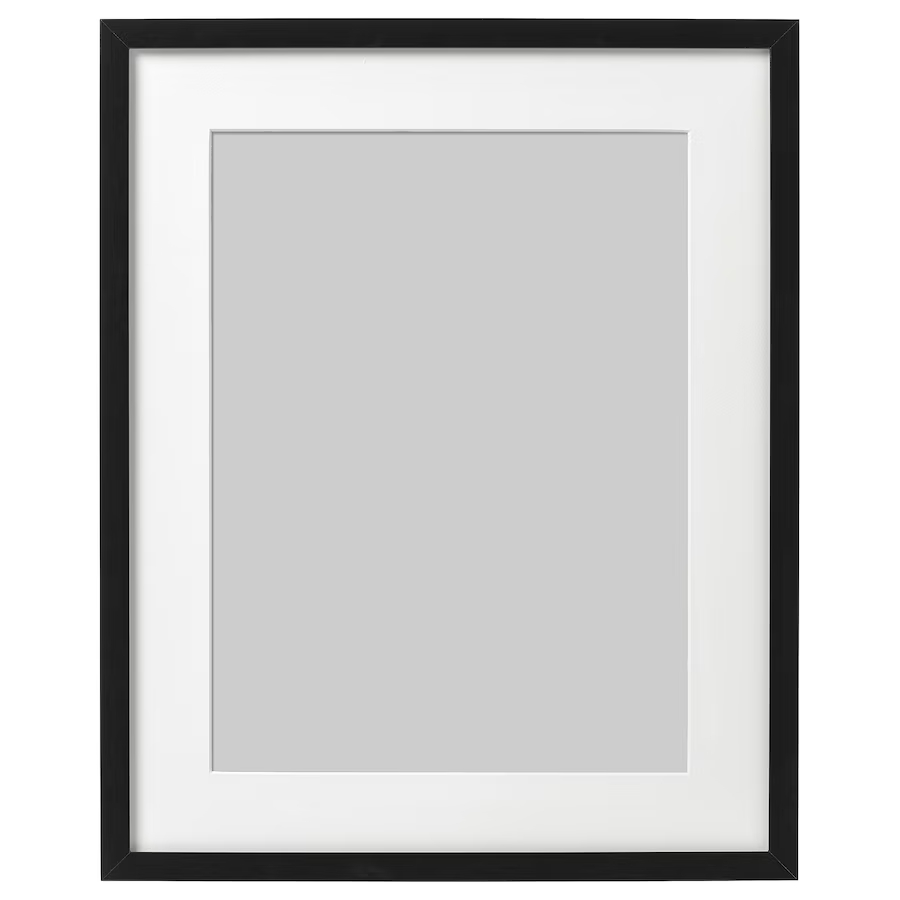
\includegraphics[width=0.5\textwidth]{images/pictureframe.jpg}
\end{center}

The frame may be empty or it may contain a picture. 

\end{frame}

\begin{frame}
\frametitle{Paging: Picture Frame}

If the picture frame is empty, all that is necessary is to put a picture in it. 

To put in a different picture, first, take out the picture that is already there. 

Taking out the picture to empty the frame is allowed, too. 

A picture is always aligned to be completely in a frame; not half in and half out. 

\end{frame}

\begin{frame}
\frametitle{Paging: Picture Frame}


Now expand this scheme by having a very long row of picture frames. 

Each frame can contain one picture at a time, at most. 

A picture can be in at most one frame at a time. 

\end{frame}

\begin{frame}
\frametitle{Paging: Process Start}

A process starts, is loaded into memory, and has initial memory requirements. \\
\quad (e.g., the stack and global variables).

The number of pages can \& will change over time as memory is allocated/freed. 

A process may also be swapped out to disk, but to run it needs to be swapped in. 

A process will take up a certain number of pages in memory at any given time.

\end{frame}

\begin{frame}
\frametitle{Page Benefits}

Pages separate the logical address from the physical address.

Programmers may pretend the address space of the computer is $2^{64}$ bytes.

Not just how many GB of memory are in the physical machine. 

\end{frame}

\begin{frame}
\frametitle{Page Example}

\begin{center}
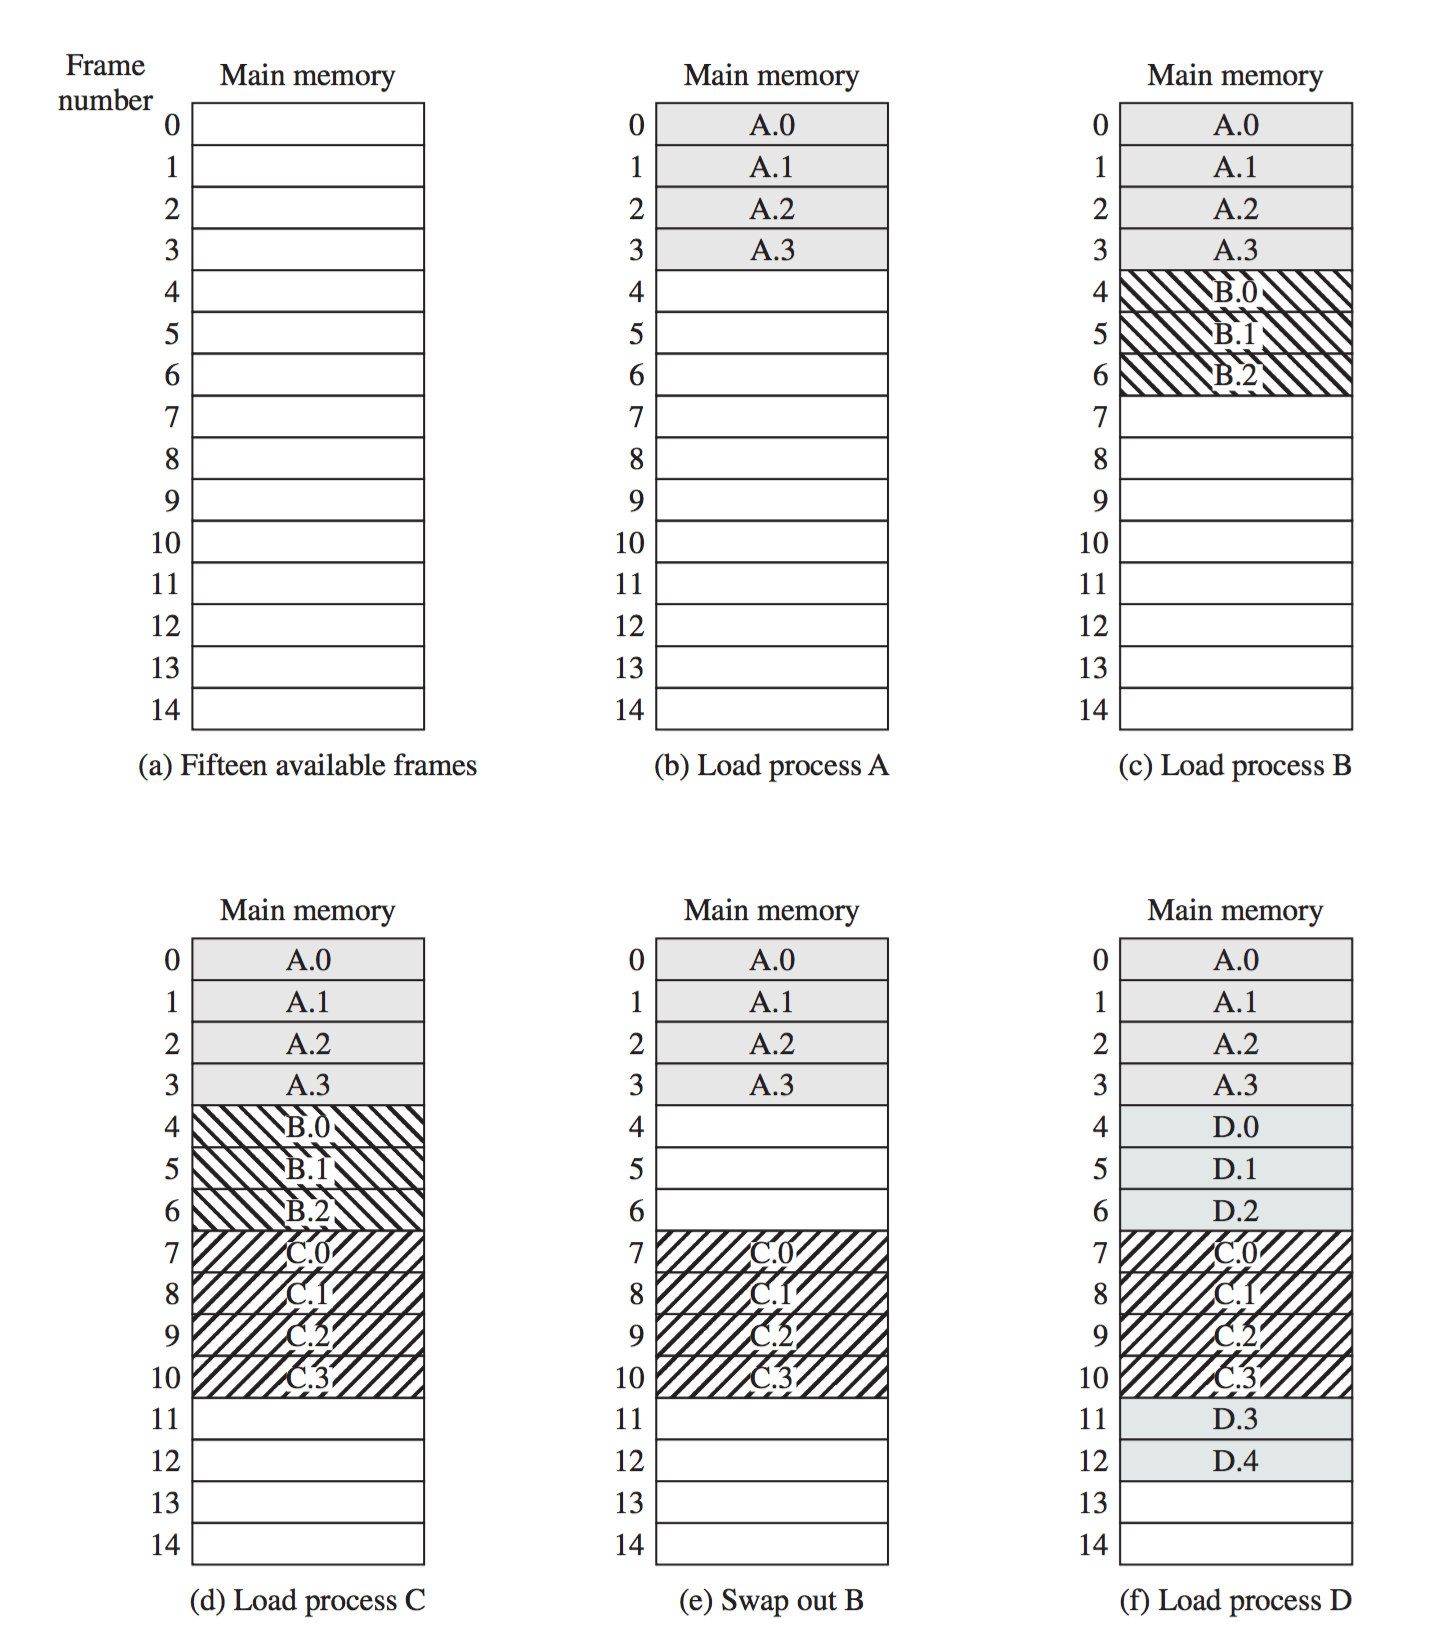
\includegraphics[width=0.6\textwidth]{images/loading-pages.png}
\end{center}


\end{frame}

\begin{frame}
\frametitle{Page Tables}

Now that we have multiple segments for each process and they are no longer contiguous, it is insufficient to have a base address and a limit.

Each process needs a page table, to keep track of which pages are located where in memory. 

A list of free frames is also necessary

\end{frame}

\begin{frame}
\frametitle{Page Table Diagram}

\begin{center}
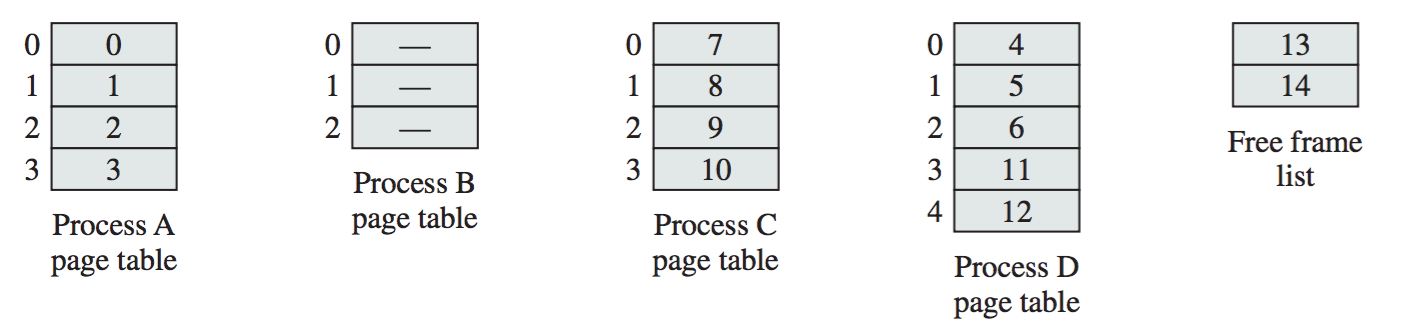
\includegraphics[width=\textwidth]{images/page-tables.png}
\end{center}


\end{frame}

\begin{frame}
\frametitle{Page Table}

The page table is used to map logical memory to physical memory.

\begin{center}
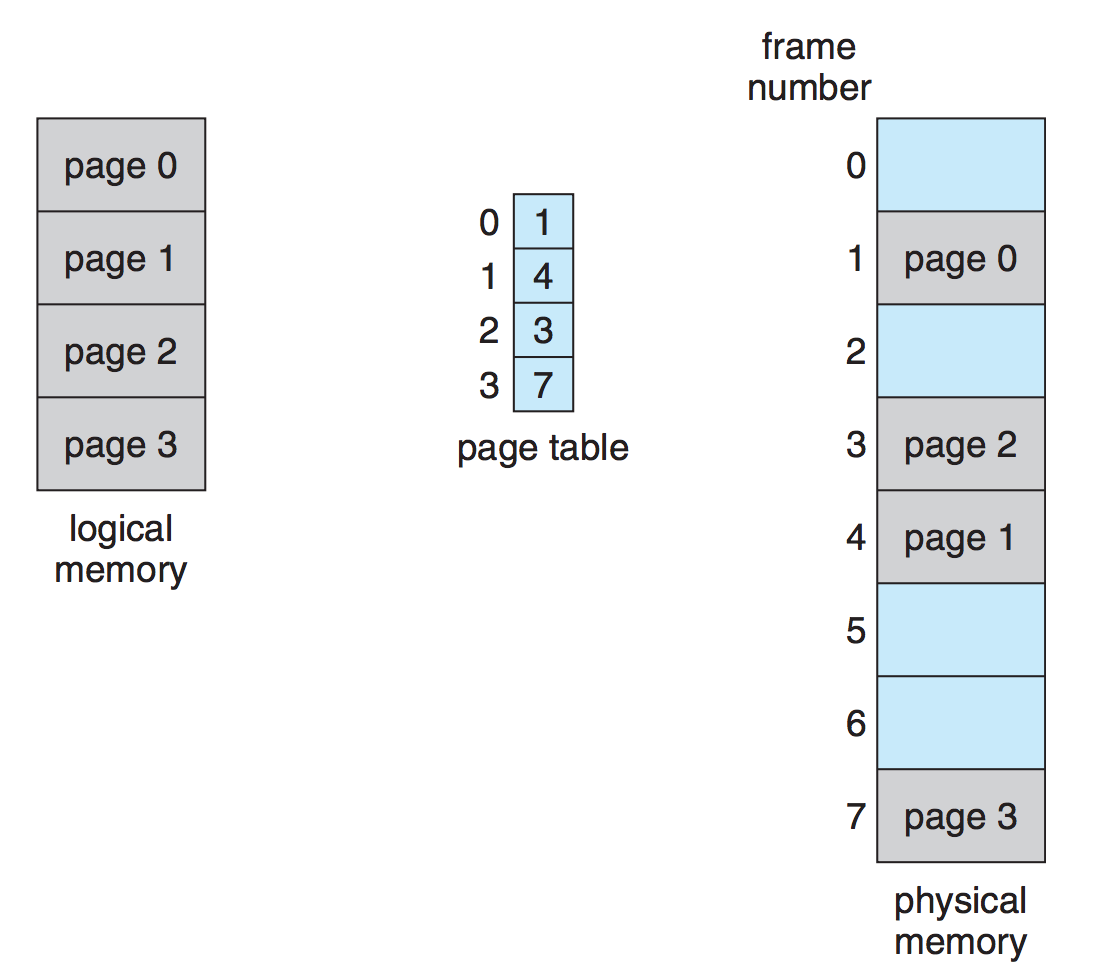
\includegraphics[width=0.65\textwidth]{images/page-table-mapping.png}
\end{center}

\end{frame}


\begin{frame}
\frametitle{Page Sizes}

For convenience, page size is usually a power of 2.\\
\quad (and the actual value is determined by hardware). 

The selection of a power of 2 makes translating a logical address into a tuple of the page number and offset easy. 

If the logical address space has size $2^{m}$ and the page size is $2^{n}$ bytes:\\
\quad The high order $m - n$ bits of the logical address are the page number;\\
\quad The lower $n$ bits are the page offset. 


\end{frame}

\begin{frame}
\frametitle{Pages: External Fragmentation}

External fragmentation is eliminated as a problem in this scheme, because pages are all the same size. 

That also means that compaction is not an issue. 

Compaction, when it's possible, is painful enough in memory. \\
\quad It is excruciating to do on disk. 

We accept some internal fragmentation because a process gets a whole page. 


\end{frame}

\begin{frame}
\frametitle{Pages: Internal Fragmentation}

How much internal fragmentation do we have to live with? Not very much. 

If the memory required aligns perfectly with a multiple of the page size, then no memory is wasted. 

If a new memory allocation comes in, then a new page is allocated and added to the logical memory space of the process. 

\end{frame}

\begin{frame}
\frametitle{Pages: Internal Fragmentation}

The last frame, however, may not be completely full. 

In the worst case scenario, a full page less one byte is wasted. 

Internal fragmentation of one page is not very much overall.


\end{frame}

\begin{frame}
\frametitle{Pages: Does Size Matter?}

How big should page sizes be? 

If they are smaller, then less memory is wasted in internal fragmentation. 

However, having a large number of pages introduces a lot of overhead. 

The size of pages has tended to grow along with the size of main memory.

\end{frame}

\begin{frame}
\frametitle{Page Size: Disk Size}

The key factor is actually disk: the disk operates on a certain block size and it is most efficient for the size of a page to be equal to a disk read/write size. 

That way when a page is to be swapped into or out of memory, it can be done in a single disk read or write. 

In a typical modern system, pages are 4~KB, but they can be bigger.

\end{frame}

\begin{frame}
\frametitle{Pages: Size and Protection}

Now we finally have a good answer to why the application developer can treat memory as if it is infinitely large and unshared. 

\begin{center}
	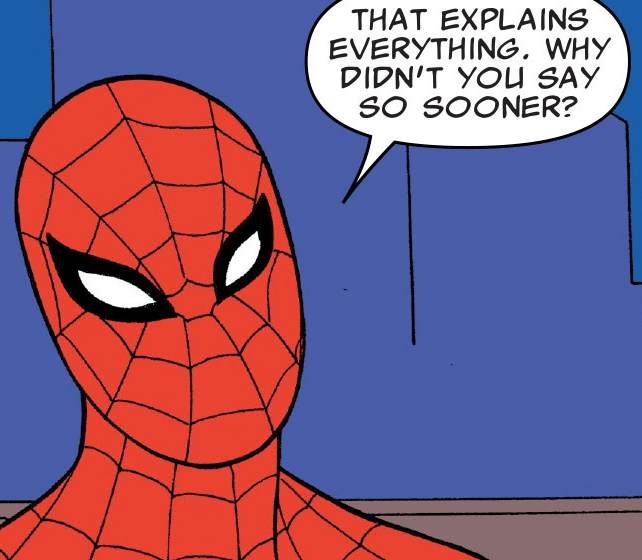
\includegraphics[width=0.5\textwidth]{images/explained.png}
\end{center}

The program is scattered across physical memory, but appears to the application developer and running application as if it is all contiguous. 

\end{frame}


\begin{frame}
\frametitle{Pages: Size and Protection}

We also get protection in this scheme.

A program cannot access any address outside of its memory space. 

There is no way to make a memory request outside of the logical memory space. 

No matter what address is generated, it could only be inside the page table, and the page table has only entries of that process.

\end{frame}

\begin{frame}
\frametitle{Pages: The OS View}

The operating system, however, can manage memory of all processes, so it will need another scheme. 

\begin{center}
	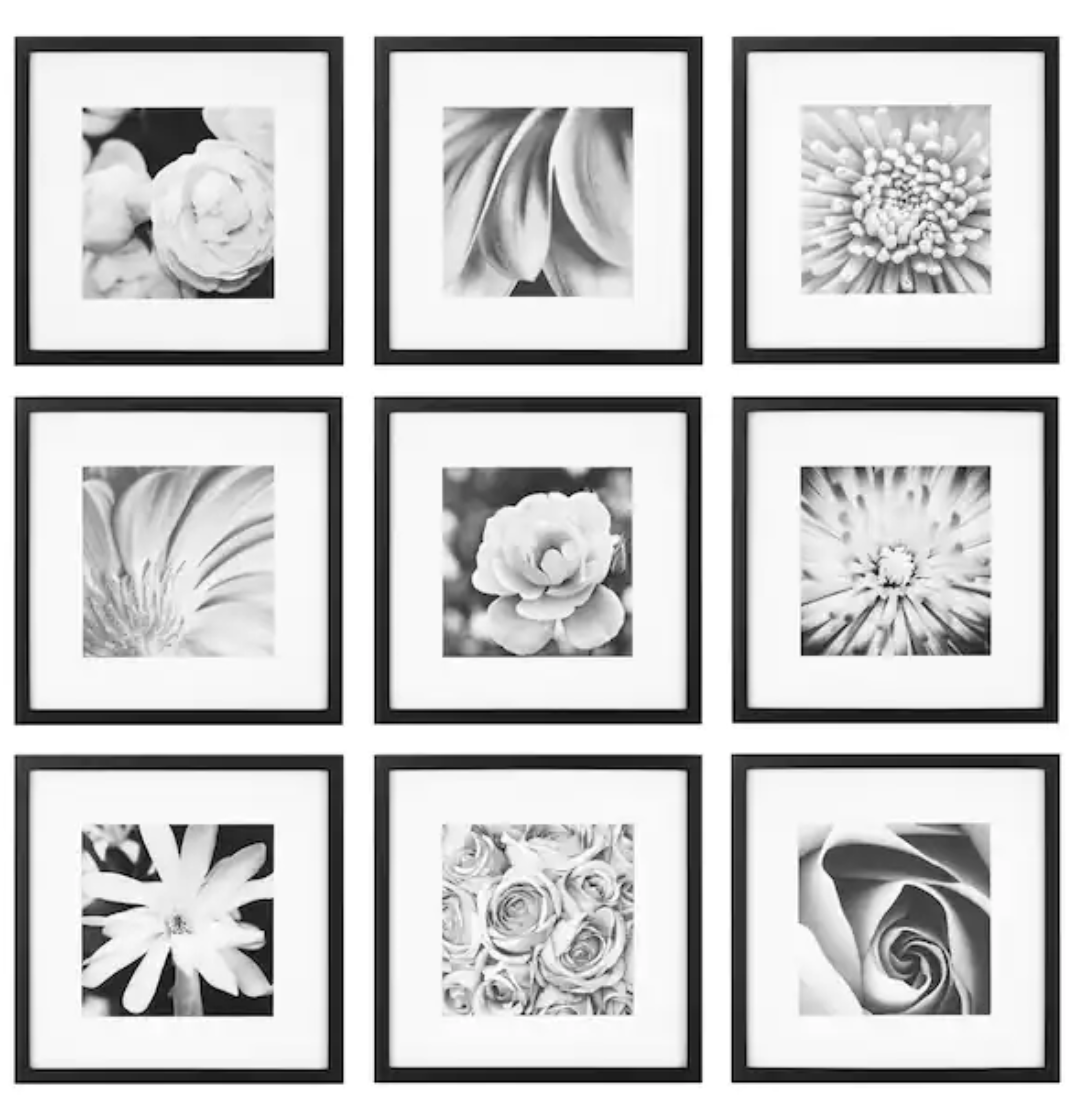
\includegraphics[width=0.4\textwidth]{images/frametable.png}
\end{center}

The OS will operate on the \alert{frame table}, a listing of all the frames, indicating which page of which process a frame currently holds, if any.


\end{frame}

\begin{frame}
\frametitle{Shared Pages}

Another great advantage of paging is the possibility of sharing of common code. 

Users very often have multiple programs open; sometimes they are duplicates.

In a multiuser system, different users may have some of the same program open.

We could reduce memory consumption if common parts of this program are shared between all instances of that program.

\end{frame}


\begin{frame}
\frametitle{Sharing is Caring: \texttt{vi}}

Imagine there are 5 users on the system, each of whom wants to use \texttt{vi}. 

Let's say the program itself uses 10 pages (made up number) on its own, and then some variable number of pages based on what file is being edited. 

Without sharing, each copy of \texttt{vi} that runs will consume 10 pages, so 50 pages are being used for the executable. 

If we can share those 10 pages, we have saved 40 pages worth of memory space.


\end{frame}

\begin{frame}
\frametitle{Sharing Code}

Other programs and code can easily be shared, such as compilers, libraries, and operating system utilities. 

In fact, any code can be shared as long as it is \alert{reentrant} (also sometimes called pure or stateless). 

This is code that does not change when it is executed. 

That means there is no state maintained by the code. 


\end{frame}

\begin{frame}[fragile]
\frametitle{Non-Reentrant Code}

Any function that accesses a global or static variable is non-reentrant.

\begin{verbatim}
int tmp;
void swap( int *x, int *y ) {
  tmp = *x;
  *x = *y;
  *y = tmp; 
}
\end{verbatim}

\end{frame}

\begin{frame}
\frametitle{Page Table Structure}

In the simplest form, the page table is just a standard table. 

This structure is simple, but page tables can be very large.

If the system is 32-bit, and page sizes are 4~KB ($2^{12}$), then the page table has $2^{32}/2^{12} = 2^{20}$ pages, or about 1 million entries.

\end{frame}

\begin{frame}
\frametitle{Page Table Structure}

We will examine three strategies for structuring the table:

\begin{enumerate}
	\item Hierarchical paging.
	\item Hashed page tables.
	\item Inverted page tables.
\end{enumerate}

\end{frame}

\begin{frame}
\frametitle{Hierarchical Paging}

Rather than have one big table, we have multiple levels in the page table. 

The page table can be broken up and need not be contiguous in memory. 

Suppose we have a two level system. 

\end{frame}

\begin{frame}
\frametitle{Hierarchical Paging}

If the page number is $p$, the first $k$ bits indicate the \alert{outer page}. 

The outer page contains some information about where the \alert{inner pages} are. 

The remaining $p-k$ bits identify the inner page. 

After the inner page is identified, the displacement $d$ is then calculated.


\end{frame}



\begin{frame}
\frametitle{Hashed Page Tables}

Instead of the page table being an array of entries, turn it into a hash table.

There is a hash function to assign pages to ``buckets'' and each bucket is implemented as a linked list. 
 
Then each element of the list is examined to find the matching page.

\end{frame}

\begin{frame}
\frametitle{Inverted Page Tables}

For 32-bit virtual addresses, a multilevel page table can work. 

But with 64-bit computers, with 4~KB pages, the page table requires $2^{52}$ entries.

If an entry is 8 bytes, then the table is over 30 million gigabytes (30~PB).

\end{frame}

\begin{frame}
\frametitle{Inverted Page Tables}

Does your computer have that much memory?\\
\quad ... If so, can I borrow it?

\begin{center}
	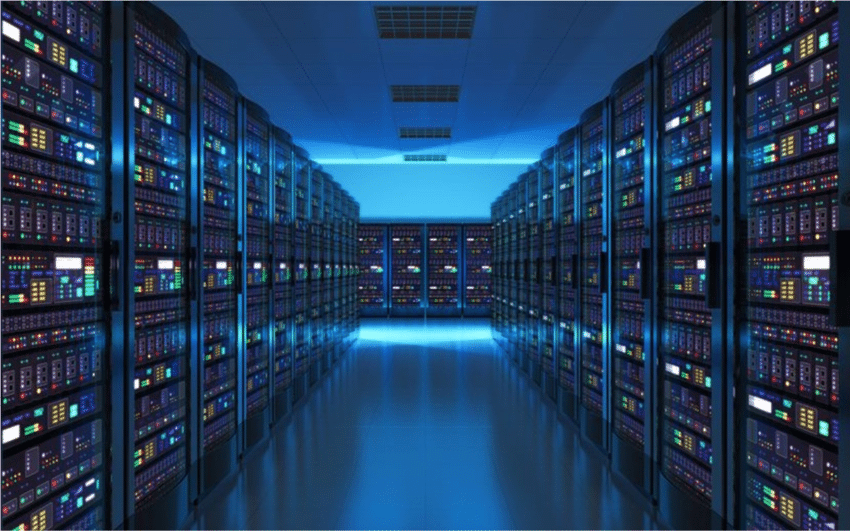
\includegraphics[width=\textwidth]{images/datacentre.png}
\end{center}



\end{frame}

\begin{frame}
\frametitle{Inverted Page Tables}

Inverted page table: one entry per frame, rather than one entry per page.

The entry keeps track of the process and page number. 

This saves a huge amount of space.\\
\quad (1~GB of ram with a 4~KB page size $\rightarrow$ page table requires only $2^{18}$ entries).

The drawback: no longer possible find physical pages by looking at the address.\\
\quad Instead, searching (slow).

\end{frame}

\begin{frame}
\frametitle{Paging: Hardware Support}

Memory accesses are very frequent and require additions and comparisons. 

Recall an operation as simple as adding two numbers requires fetching the add instruction, fetching the operands, and storing the result. 

To prevent abysmal performance, modern computers have hardware support.

Hardware is much, much faster than doing these operations in software.



\end{frame}

\begin{frame}
\frametitle{Paging: Hardware Support}

The simplest implementation is to use a set of dedicated registers.

Registers are the fastest form of storage. 

When a process switch takes place, these registers, just as all other registers, are replaced with those of the process to run. 

The PDP-11 was an example of a system that had this architecture.\\
\quad Addresses were 16 bits and the page size was 8~KB.

\end{frame}

\begin{frame}
\frametitle{Paging: Hardware Support}

The page table was therefore 8 entries and kept in fast registers. 

This might work if the number of entries in the page table is small (~256 entries). 

The page table can easily be something like 1 million entries.\\
\quad Does your CPU have 1 million registers? If so...?

The page table is in main memory. A single register points to the page table.


\end{frame}

\begin{frame}
\frametitle{There's Always a Catch}

To access a page from memory, we need to first figure out where it is, so that requires accessing the page table in main memory. 

Then after retrieving that, we can look in the page table to find the frame where the desired page is stored. 

Then we can access that page. 

\end{frame}

\begin{frame}
\frametitle{There's Always a Catch}

So two memory accesses are required for every read or write operation. 

As far as the CPU is concerned, main memory already moves at a snail's pace. 

Doubling the amount of time it takes to do a read or write means it takes roughly forever. 

Thus, we will need to find a way to speed this up.

\end{frame}

\begin{frame}
\frametitle{Hardware to the Rescue, Again}

A fast cache called the \alert{translation lookaside buffer} (TLB). 

You can think of the TLB as a key-value pair (think HashMap). 

The key is the logical address and the value is the physical address. 

\end{frame}

\begin{frame}
\frametitle{Translation Lookaside Buffers}

To make the search fast, the comparison is done on all items simultaneously. 

To prevent this from being extremely expensive, the size of the TLB is limited.

It's usually something around 32 to 1024 entries in size. 

Systems have evolved from having no TLBs to having multiple levels, over time.

\end{frame}


\begin{frame}
\frametitle{Check the TLB}

When a memory read/write is issued, the page number is checked.

If it is found in the TLB then the frame number is immediately known. 

If the page number is not found in the TLB, this is what we call a \alert{TLB miss}.

We must look in the full page table, which unfortunately is slower because it requires reading from memory.

\end{frame}

\begin{frame}
\frametitle{TLB Operation}

\begin{center}
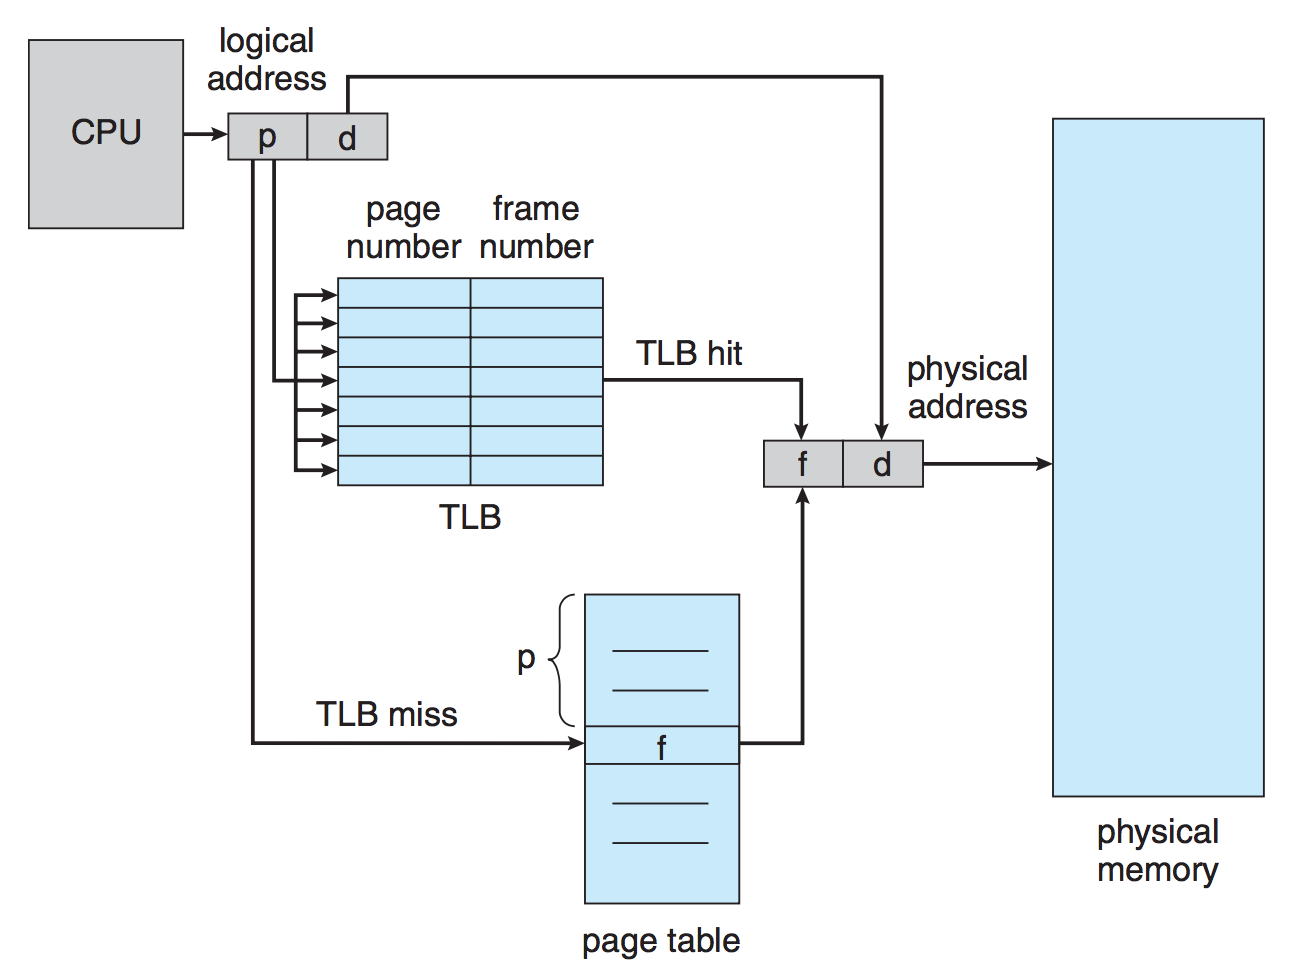
\includegraphics[width=0.9\textwidth]{images/tlb-hardware.png}
\end{center}


\end{frame}

\begin{frame}
\frametitle{Caching}

The TLB idea is another instance of the strategy of caching. 

We talked about that earlier on in our discussion about memory.\\
\quad Everything we learned there applies here too!

\end{frame}

\end{document}

